%% LaTeX-Beamer template for KIT design
%% by Erik Burger, Christian Hammer
%% title picture by Klaus Krogmann
%%
%% version 2.1
%%
%% mostly compatible to KIT corporate design v2.0
%% http://intranet.kit.edu/gestaltungsrichtlinien.php
%%
%% Problems, bugs and comments to
%% burger@kit.edu

\documentclass[18pt]{beamer}
\usepackage[utf8]{inputenc}

%% SLIDE FORMAT

% use 'beamerthemekit' for standard 4:3 ratio
% for widescreen slides (16:9), use 'beamerthemekitwide'

\usepackage{templates/beamerthemekit}
% \usepackage{templates/beamerthemekitwide}

\usepackage{graphicx}

%% TITLE PICTURE

% if a custom picture is to be used on the title page, copy it into the 'logos'
% directory, in the line below, replace 'mypicture' with the
% filename (without extension) and uncomment the following line
% (picture proportions: 63 : 20 for standard, 169 : 40 for wide
% *.eps format if you use latex+dvips+ps2pdf,
% *.jpg/*.png/*.pdf if you use pdflatex)

%\titleimage{mypicture}

%% TITLE LOGO

% for a custom logo on the front page, copy your file into the 'logos'
% directory, insert the filename in the line below and uncomment it

%\titlelogo{mylogo}

% (*.eps format if you use latex+dvips+ps2pdf,
% *.jpg/*.png/*.pdf if you use pdflatex)

%% TikZ INTEGRATION

% use these packages for PCM symbols and UML classes
% \usepackage{templates/tikzkit}
% \usepackage{templates/tikzuml}

% the presentation starts here

\title[Graph von Ansicht]{Graph von Ansicht:\\ Visualisierung von Programmabhängigkeitsgraphen}
\subtitle{}
\author{Nicolas Boltz, Jonas Fehrenbach, Sven Kummetz, Jonas Meier, Lucas Steinmann}

\institute{}

% Bibliography

\bibliographystyle{plain}
\graphicspath{{resourcen/}}
%\usepackage[citestyle=authoryear,bibstyle=numeric,hyperref,backend=biber]{biblatex}
%\addbibresource{templates/example.bib}
%\bibhang1em

\begin{document}

% change the following line to "ngerman" for German style date and logos
\selectlanguage{ngerman}

%title page
\begin{frame}
\titlepage
\end{frame}

\author{Nicolas B., Jonas F., Sven K., Jonas M., Lucas S.}
%table of contents
\begin{frame}{Gliederung}
\tableofcontents
\end{frame}

\section{Einleitung/Zielbestimmung}
\begin{frame}{Ziele}
\begin{itemize}
\item anpassbare Visualisierung von Graphen
\pause
\item Betrachtung und Analyse visualisierter Graphen.
\pause
\item Erweiterbarkeit durch Plugins (Bsp Joana)
\pause
\item laden und Speichern gängiger Dateiformate (Bsph SVG und GML)
\pause
\item eine an Joana angepasste Visualisierung (als Plugin)
\end{itemize}
\end{frame}

\section{Benutzerschnittstellen}
\begin{frame}{Benutzerschnittstellen}
\begin{tabular}{cc}

    \begin{minipage}{0.45\textwidth}
    Kommandozeile \\
    \raisebox{-.5\height}{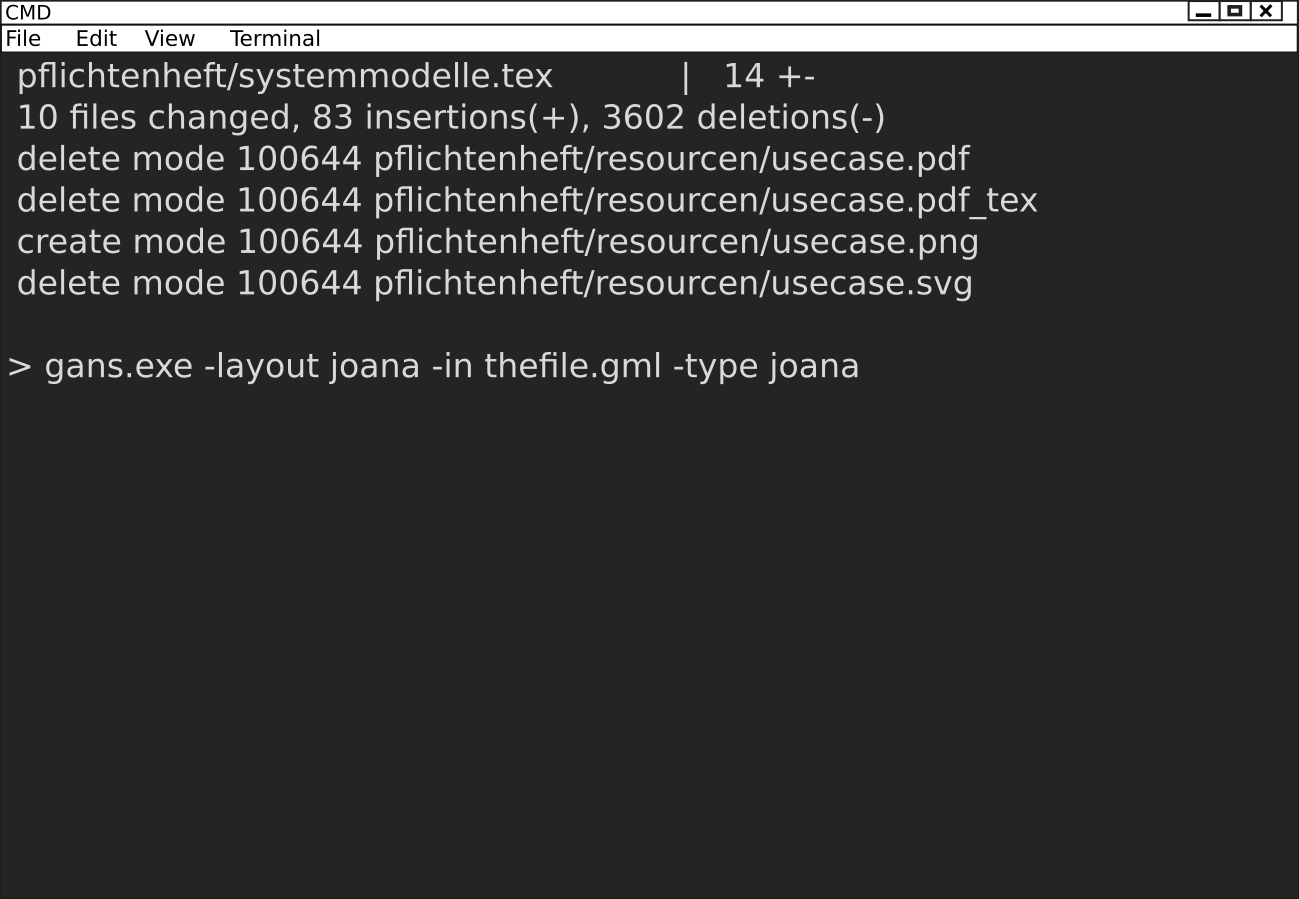
\includegraphics[width=150pt]{resourcen/cmd.png}}

    \begin{itemize}
      \item schnelle Möglichkeit Graphen zu layouten
      \pause
      \item Massenverarbeitung von Dateien
      \pause
    \end{itemize}
    
    \end{minipage}
  \pause
  &

    \begin{minipage}{0.45\textwidth}
     GUI \\
    \raisebox{-.5\height}{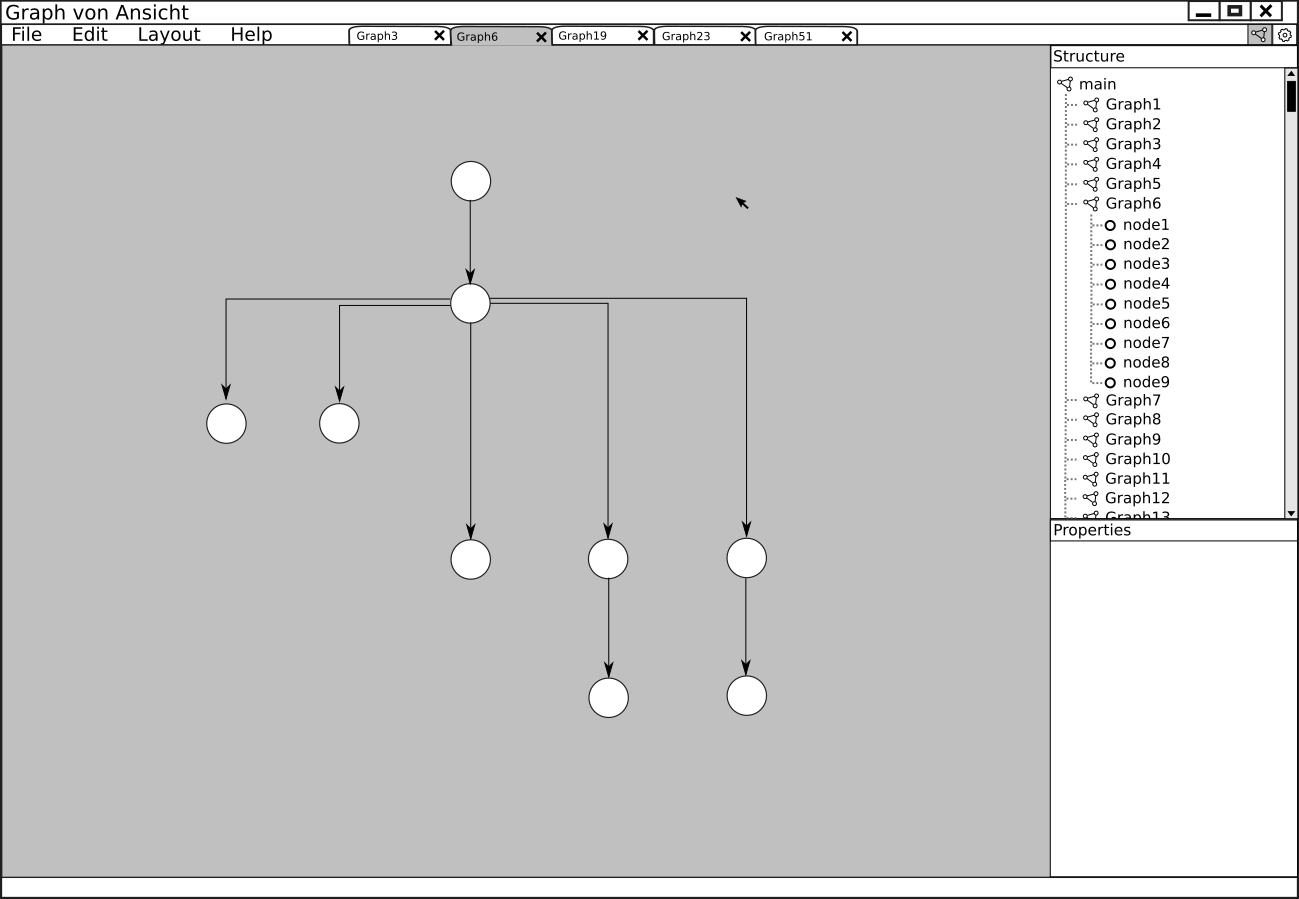
\includegraphics[width=150pt]{resourcen/gui.png}}

    \begin{itemize}
      \item interaktives Interface
      \pause
      \item Darstellung der Graphen
      \pause
      \item höhere Anpassbarkeit (ohne ein Plugin zu programmieren)
      \pause
    \end{itemize}

    \end{minipage}
  \\

\end{tabular}
\end{frame}

\section{Szenario}
\begin{frame}{Szenario}
\begin{itemize}
	% Wissenschaftlicher Mitarbeiter möchte den Unterschied eines möglichen Informationslecks im Programmablauf
	% zwischen zwei Änderungen in einem Programm visuell darstellen(Für Paper, Artikel, oder z.B. Lehre)
	\item Importieren der JOANA-Datei %eines Programms das analysiert werden soll
	\pause
	\item Pfad im Callgraphen verfolgen und/oder Methodengraph öffnen
	\pause
	\item Anpassen der Ansicht des Graphen % Einklappen uninteressanter Knoten und Constraint zur übersichtlichen Darstellung der interessanten Knoten hinzufügen
	\pause
	\item Exportieren der Ansicht im SVG-Format
	\pause
	\item Informationsleck in der Anwendung schließen % und von JOANA analysieren lassen
	\pause
	\item Importieren und betrachten der gemachten Änderung % an dem zuvor betrachteten Aufruf oder Methode in Graph von Ansicht 
	\pause
	\item Anpassen der Ansicht des Graphen % Einklappen uninteressanter Knoten und Constraint zur übersichtlichen Darstellung der interessanten Knoten hinzufügen
	\pause
	\item Exportieren der Ansicht im SVG-Format
	\pause
	%Einfügen der Grafiken in ein Paper oder wissenschaftlichen Artikel zur Verdeutlichung eines bestimmten Problems und/oder dessen Lösung
\end{itemize}	
\end{frame}

\section{Weitere Funktionen}
\begin{frame}{Funktionsübersicht}
\begin{itemize}
\item Graph Visualisierung mittels Sugiyama Framework
\pause
\item Callgraph Layout
\pause
\item Navigation in der Darstellung des Graphen
\pause
\item anpassbare Einstellung der Darstellung
\pause
\item Graph Visualisierung mittels Sugiyama Framework
\pause
\item Informationsanzeige zu Knoten und Kanten
\pause
\item Statistiken des Graphen
\pause
\item filtern bestimmter Knoten und Kanten in der Ansicht
\pause
\item Mehrere Graphen gleichzeitig betrachtbar
\pause
\end{itemize}
\end{frame}

\section{Erweiterbarkeit}
\begin{frame}{Pluginschnittstellen}
\end{frame}
\appendix
\beginbackup

\begin{frame}[allowframebreaks]{References}
\bibliography{templates/example}
\end{frame}

\backupend

\end{document}
